
%%%%%%%%%%%%%%%%%%%%%%%%%%%%%%%%%%%%%%%%%%%%%%%%%%%%%%%%%%%%%%%%
%%%%%%%%%%%%% Efficient video features
%%%%%%%%%%%%%%%%%%%%%%%%%%%%%%%%%%%%%%%%%%%%%%%%%%%%%%%%%%%%%%%%
\section{Efficient video features}
\label{sec:features}

Dense Trajectory (DT) features together with MBH and HOF descriptors achieve state-of-the-art accuracy in action recognition~\cite{Wang12} at the cost of high computational requirements.
%but are limited in speed with the current implementation being able to process one or a few frames per second depending on video resolution. 
%Currently available implementation of Dense Trajectory (DT) features provided by the authors of~\cite{Wang12} can process approximately one video frame per second. 
The analysis in~\cite{Wang12} indicates that most of the running time ($61\%$) is spent on the computation of optical flow, while the second most expensive operation ($36\%$) is aggregation of dense flow measurements into histogram descriptors (discarding the "save features to disk" part). In this paper we alleviate the expense of both of these steps by (i) re-using motion estimates available from video compression and (ii) constructing descriptors from very sparse motion measurements. %, typically available only on a $16\times16$ pixel grid in standard video compression schemes.
In this section we first analyze the quality of motion vectors available in compressed video representations and then describe our efficient video descriptor.

%This section describes and motivates the design of our video descriptor. We first review existing descriptors and outline their strengths and limitations. We then analyze the properties of the motion field available in compressed video representations and use it to construct a new video descriptor.

%\subsection{Local video descriptors}

%Local video descriptors~\cite{Dollar05,Laptev05,Schuldt04} have been shown successful for recognizing events in realistic videos such as movies and TV footage. Several descriptors have been proposed capturing local histograms of 2D gradients (HOG) and flow orientations(HOF)~\cite{Laptev08}, histograms of 3D gradients (HOG3D)~\cite{Scovanner07,klaser2008spatio}, motion boundary histograms (MBH)~\cite{Dalal06,Wang12}, local shapes of point trajectories~\cite{Matikainen09,Messing09,Wang12} and local trinity patterns~\cite{Yeffet09,Kliper12}. Intermediate-level features such as attributes~\cite{Liu11} and pre-trained action bank detectors~\cite{Sadanand12} have also been explored. Recent comprehensive evaluation~\cite{Wang12} suggests that MBH, HOF and HOG descriptors densely sampled along point trajectories result in excellent performance and outperforms other methods on a large number of existing action recognition benchmarks. In particular, as we re-confirm in Section~\ref{sec:experiments}, MBH and HOF motion descriptors provide crucial contributions to the recognition performance.




\begin{figure*}[t!]
\begin{center}
\hspace*{-.3cm}
\begin{tabular}{p{.45\textwidth}p{.5\textwidth}p{.05\textwidth}}
\mbox{}\vspace{-2.5cm}\newline
\hspace*{1cm}{\small Sample frame from MPI Sintel dataset~\cite{Butler12}}\vspace{.07cm}\newline
%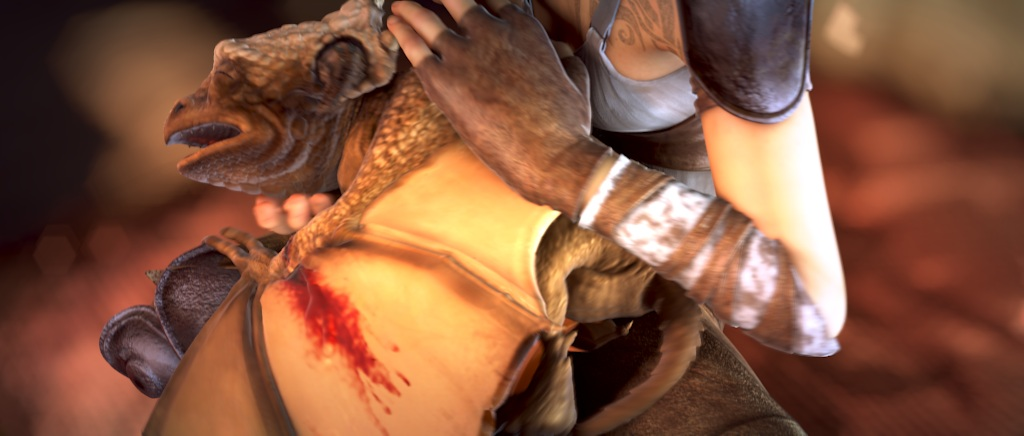
\includegraphics[trim=2cm 0cm 3cm 0cm, clip=true, width=.85\linewidth]{cvpr14_figures/flow/bandage_1_frame_0010.jpg}$\,\,$
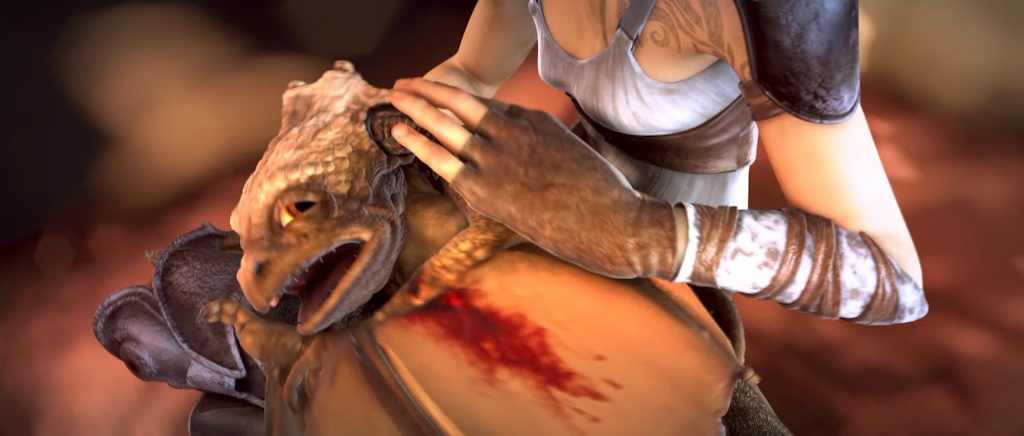
\includegraphics[trim=2cm 0cm 3cm 0cm, clip=true, width=.95\linewidth]{cvpr14_figures/flow/bandage_1_frame_0020.jpeg}$\,\,$
&
\hspace*{-.9cm}
\begin{tabular}{cc}
\small Quantized ground truth flow & \small Quantized MPEG flow, err=$0.283$\\
%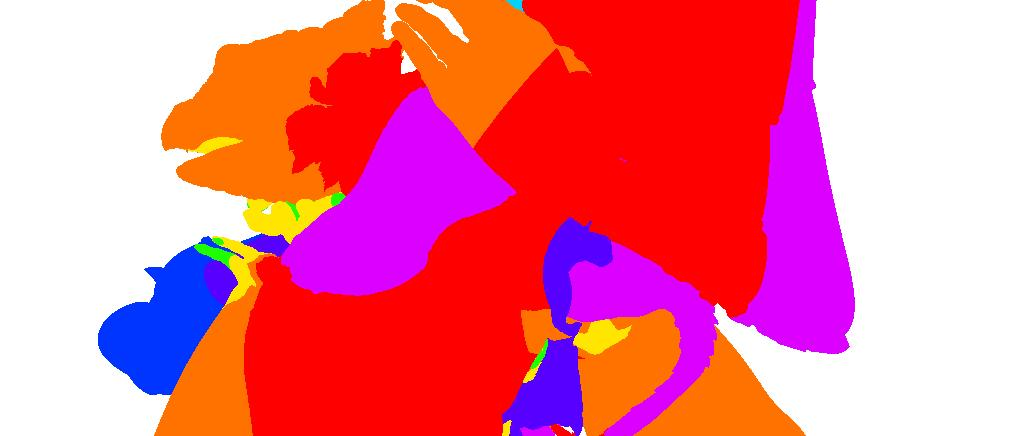
\includegraphics[width=.4\linewidth]{cvpr14_figures/flow/flow_bandage_1_frame011_orig_quant.jpeg} \vspace{.05cm}&
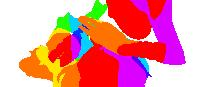
\includegraphics[width=.45\linewidth]{cvpr14_figures/flow/flow_bandage_1_frame021_orig_quant.jpeg} \vspace{.05cm}&
%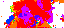
\includegraphics[width=.4\linewidth]{cvpr14_figures/flow/flow_bandage_1_frame011_mpeg_quant.png}  \vspace{.05cm}\\
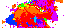
\includegraphics[width=.45\linewidth]{cvpr14_figures/flow/flow_bandage_1_frame021_mpeg_quant.png}  \vspace{.05cm}\\
\small Quant. LK flow, err=$0.334$ & \small Quant. Farneb\"ack flow, err=$0.286$ \\
%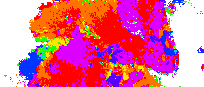
\includegraphics[width=.4\linewidth]{cvpr14_figures/flow/flow_bandage_1_frame011_stip_quant.png}  \vspace{.05cm}&
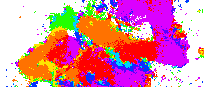
\includegraphics[width=.45\linewidth]{cvpr14_figures/flow/flow_bandage_1_frame021_stip_quant.png}  \vspace{.05cm}&
%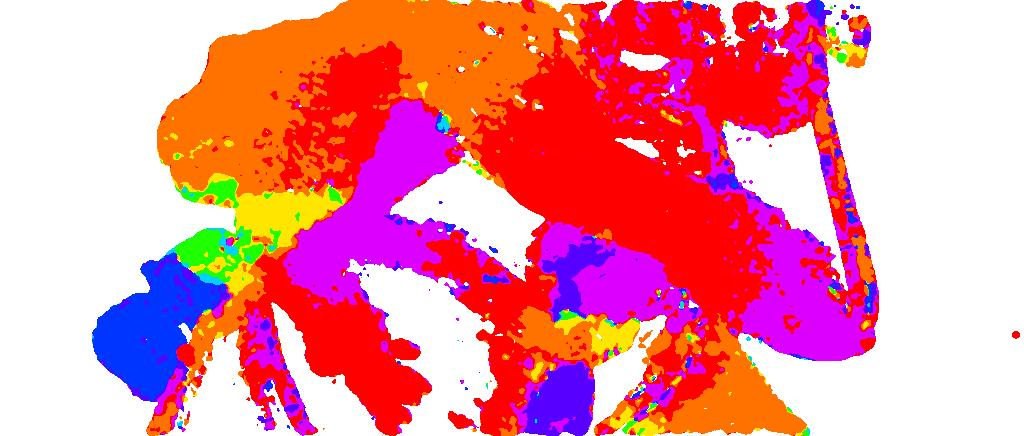
\includegraphics[width=.4\linewidth]{cvpr14_figures/flow/flow_bandage_1_frame011_traj_quant.jpeg} \vspace{.1cm}\\
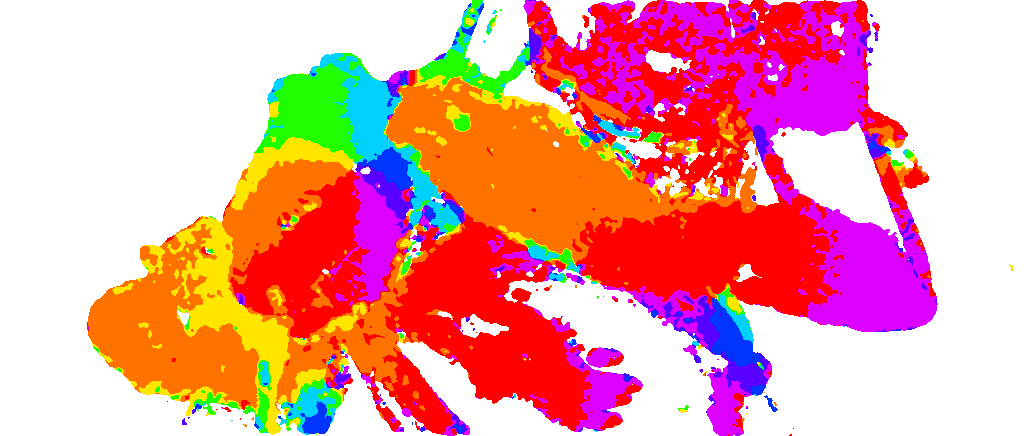
\includegraphics[width=.45\linewidth]{cvpr14_figures/flow/flow_bandage_1_frame021_traj_quant.png} \vspace{.1cm}\\
\end{tabular}
&
\mbox{}\vspace{1cm}\newline
\hspace*{-1.1cm}
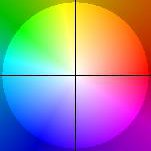
\includegraphics[width=1\linewidth]{cvpr14_figures/flow/flowcolorcode_reoriented.jpg}\vspace{.05cm}
\end{tabular}
\caption[Comparison of optical flow estimation]{Comparison of optical flow estimation for a synthetic video sequence ``bandage\_1'' from MPI Sintel dataset~\cite{Butler12}. On the right we compare the ground truth flow with the flow obtained from DivX video compression (MPEG flow) as well as optical flow estimated with Lukas-Kanade~\cite{Lucas81} and Farneb\"ack~\cite{Farneback03} methods. The direction of flow vectors is quantized into eight equally distributed orientations and is color-coded according to the color-wheel on the bottom-right. White color represents no motion. The error of the flow is obtained by the ratio of incorrectly quantized flow values when compared to the ground truth and evaluated over the whole video. While the resolution of MPEG flow is lower compared to other methods, the accuracy of all three methods is comparable both quantitatively and qualitatively.
%Left, top-to-bottom: ground truth flow; motion vectors from MPEG4 video compression; Lukas-Kanade flow (EPE)~\cite{Lucas81} and Farneb\"ack flow~\cite{Farneback03}. The accuracy of MPEG4, LK and Farneb\"ack motion fields are evaluated using endpoint error~\cite{Otte94}. Right: motion estimates quantized into eight orientation bins and one ``no-motion'' bin. Error indicates the mean disagreement of quantization between ground truth flow and the three flow estimates. Note that the EPE and the quantization error of MPEG4 flow are comparable to the errors of optical flow algorithms. The flow is color-coded according to the color-wheel on the top-right.
}
%\mbox{}\vspace{-.6cm}\\
\label{fig:flow1}
\end{center}
\end{figure*}


\begin{figure*}[t!]
\begin{center}
\hspace*{-.2cm}
\begin{tabular}{cccc}
\small Original movie frame & \small Quantized MPEG flow & \small Quantized LK flow & \small Quantized Farneb\"ack flow \\
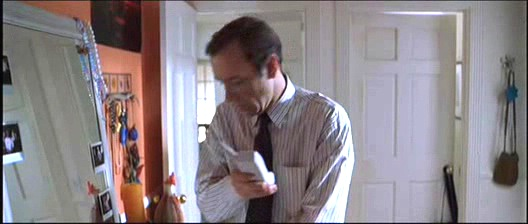
\includegraphics[width=.23\textwidth]{cvpr14_figures/flow/actioncliptrain00009_0010bright.jpg} &
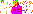
\includegraphics[width=.23\textwidth]{cvpr14_figures/flow/flow_actioncliptrain00009_frame010_mpeg_quant.png} & 
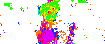
\includegraphics[width=.23\textwidth]{cvpr14_figures/flow/flow_actioncliptrain00009_frame010_stip_quant.png} &
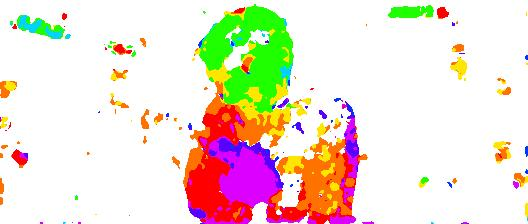
\includegraphics[width=.23\textwidth]{cvpr14_figures/flow/flow_actioncliptrain00009_frame010_traj_quant.jpeg}\\
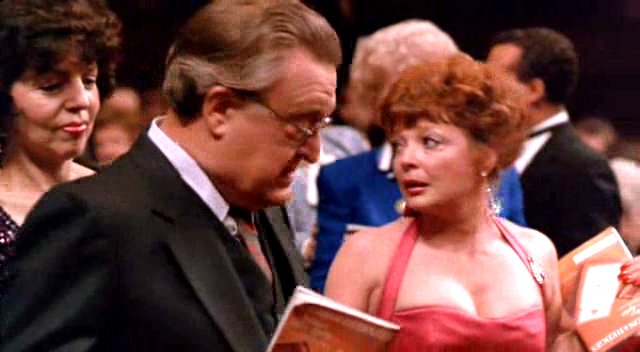
\includegraphics[width=.23\textwidth]{cvpr14_figures/flow/flow_actioncliptest00686_frame010.jpeg} & 
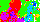
\includegraphics[width=.23\textwidth]{cvpr14_figures/flow/flow_actioncliptest00686_frame010_mv_quant.png} & 
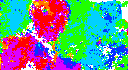
\includegraphics[width=.23\textwidth]{cvpr14_figures/flow/flow_actioncliptest00686_frame010_stip_quant.png} & 
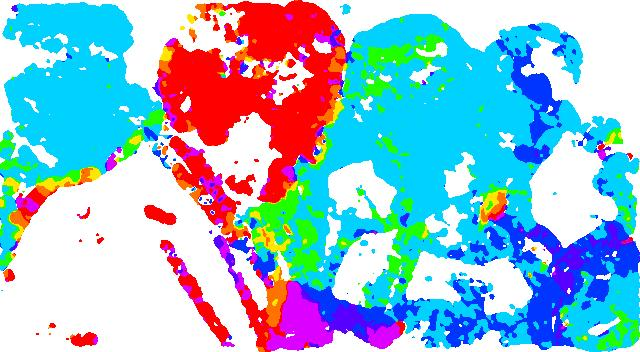
\includegraphics[width=.23\textwidth]{cvpr14_figures/flow/flow_actioncliptest00686_frame010_traj_quant.jpeg} \\
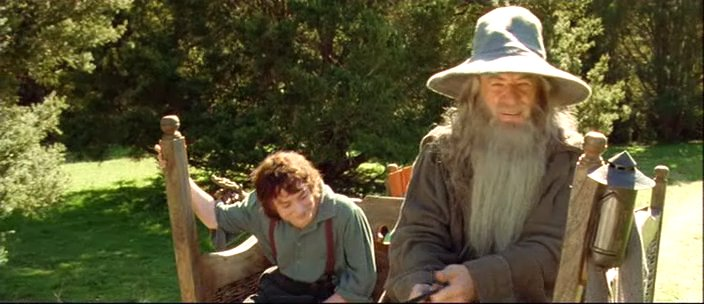
\includegraphics[width=.23\textwidth]{cvpr14_figures/flow/flow_actioncliptest00538_frame014.jpeg} & 

\includegraphics[width=.23\textwidth]{cvpr14_figures/flow/flow_actioncliptest00538_frame014_mv_quant.png} & 
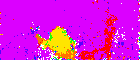
\includegraphics[width=.23\textwidth]{cvpr14_figures/flow/flow_actioncliptest00538_frame014_stip_quant.png} & 
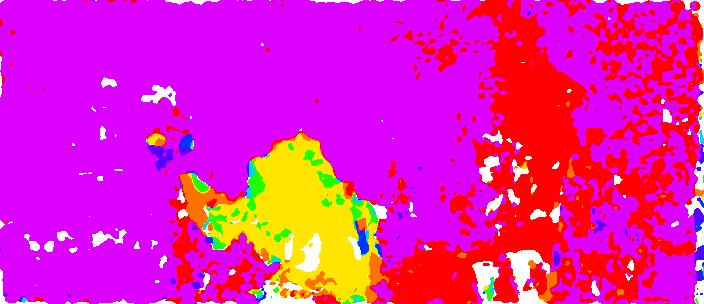
\includegraphics[width=.23\textwidth]{cvpr14_figures/flow/flow_actioncliptest00538_frame014_traj_quant.jpeg} \\
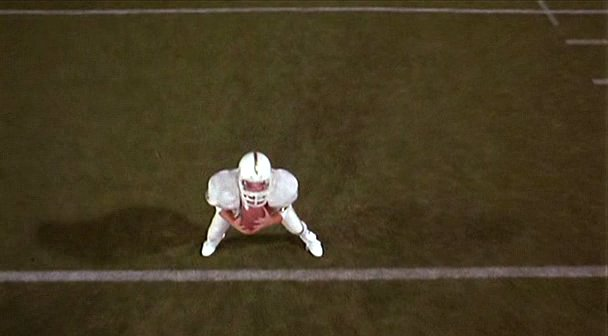
\includegraphics[width=.23\textwidth]{cvpr14_figures/flow/flow_actioncliptest00870_frame013.jpeg} & 

\includegraphics[width=.23\textwidth]{cvpr14_figures/flow/flow_actioncliptest00870_frame014_mv_quant.png} & 
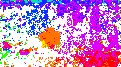
\includegraphics[width=.23\textwidth]{cvpr14_figures/flow/flow_actioncliptest00870_frame013_stip_quant.png} & 
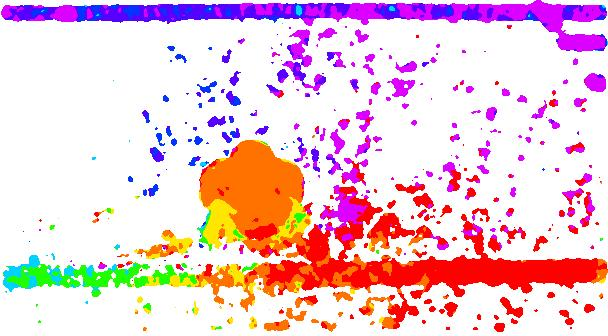
\includegraphics[width=.23\textwidth]{cvpr14_figures/flow/flow_actioncliptest00870_frame013_traj_quant.jpeg} \vspace{.2cm}\\
\end{tabular}
\caption[Qualitative comparison of optical flow]{Qualitative comparison of optical flow in real movie frames using flow estimation methods in Figure~\ref{fig:flow1}. All methods produce noisy flow estimates. Quantized values of MPEG flow are consistent with the quantized output of the two optical flow algorithms. We compare quantized flow values since these are used in descriptor computation by our and other methods.\vspace{-.3cm}}
\label{fig:flow2}
\end{center}
\end{figure*}



\subsection{Motion fields from video compression}
Consequent video frames are highly redundant with most of the changes between frames typically originating from the object or camera motion. As the storage of sparse motion vectors is much more efficient compared the storage of pixel values, video compression schemes heavily rely on motion estimation and encode coarse motion information in compressed video representations such as MPEG. This motion field can be accessed at the time of video decompression without additional cost\footnote{Full video decompression may not be required.}. %to access motion information. We currently perform full video decompression due to implementation reasons, however, it could be changed, resulting in additional speed-up of our method in the future.}.

Motion estimation by video encoders is designed to optimize video compression size and may not necessarily correspond to the true motion in the video. To verify the quality of the motion field obtained from video compression (here called MPEG flow), we compare it with the ground truth flow as well as with the output of optical flow methods by Lucas and Kanade~\cite{Lucas81} and Farneb\"ack~\cite{Farneback03}. We choose these two methods since they are deployed in existing implementations of local motion descriptors~\cite{Laptev08} and~\cite{Wang12} which we use in this work for comparison. Figure~\ref{fig:flow1} illustrates the ground truth flow and automatic flow estimates obtained for a synthetic video sequence from the recent MPI Sintel dataset~\cite{Butler12}. For this experiment we quantize flow fields into eight orientation values and one ``no-motion'' bin since this representation of flow is used in this paper for the construction of our fast video descriptor. The details and measurement results are in Figure~\ref{fig:flow1}.

%difference in flow by comparing flow estimates with the ground truth using end point error (EPE), see Figure~\ref{fig:flow1}(left). In Figure~\ref{fig:flow1}(right) we show flow fields discretized into eight orientation bins and one ``no-motion'' bin\footnote{``No-motion'' bin represents motion vectors with the magnitude below $0.4$ pixels.}. Comparing consistency of this quantization is interesting as we use it later for constructing histogram-based local motion descriptors. 

We have evaluated quantitative performance of MPEG flow in the standard Clean setup of the MPI Sintel benchmark. Despite the fact that the motion field obtained from MPEG flow has low resolution, the obtained results (EPE all=11.148 and EPE matched=6.706) outperform several methods reported on the MPI Sintel web-page {\small \url{http://sintel.is.tue.mpg.de/results}}. Qualitatively, the level of noise in MPEG flow and optical flow estimates is comparable both for synthetic and real video examples as illustrated in Figure~\ref{fig:flow2}. This indicates that the substitute of the slow optical flow used in video descriptors~\cite{Laptev08,Wang12} by the ``virtually free'' MPEG flow may not have large implications on the performance of subsequent recognition steps.


%094fad32-4801-11e1-8d64-f0def1b7a4f4



%MPEG flow
%overall EPE error 4.559; overall mag 4.981
%overall quantization error 0.196 (5bins); quantization error 0.283 (9bins)
%
%LK flow (in STIP)
%overall EPE error 4.949; overall mag 5.344
%overall quantization error 0.256 (5bis); quantization error 0.334 (9bins)
%
%DT flow
%overall EPE error 3.192; overall mag 5.334
%overall quantization error 0.214 (5bins); quantization error 0.286 (9bins)




\subsection{MPEG flow video descriptor}
\label{sec:CDdescriptor}

We follow the design of previously proposed local space-time descriptors~\cite{Laptev08,Wang12} and define our descriptor by histograms of MPEG flow vectors accumulated in a video patch. Each patch is divided into cells as illustrated in Figure~\ref{fig:CDdescriptor} and the normalized histograms from patch cells are concatenated into a descriptor vector. Constrained by the coarse $16\times16$ pixel spatial resolution of MPEG flow, we align descriptor grid cells with positions of motion vectors (red points in Figure~\ref{fig:CDdescriptor}). We also use bilinear interpolation of flow and increase the spatial resolution of the flow field by the factor of two (yellow points in Figure~\ref{fig:CDdescriptor})\footnote{We found interpolation of the flow to be important in our experiments}. 

Following~\cite{Wang12}, we compute HOF descriptors as histograms of MPEG flow discretized into eight orientation bins and a no-motion bin. For MBHx and MBHy descriptors the spatial gradients of the $v_x$ and $v_y$ components of the flow are similarly discretized into nine orientation bins. %We compute HOF, MBHx, MBHy histograms by accumulating quantized flow values within each cell (see Figure~\ref{fig:CDdescriptor}). 
The final descriptor is obtained by concatenating histograms from each cell of the $2\times2\times3$ descriptor grid followed by $l_2$-normalization of every temporal slice. HOG descriptors are computed at the same sparse set of points.

The above scheme defines a $32\times32\times15$ pixel descriptor which we compute at every location of the video defined by the spatial stride of $16$ pixels and temporal stride of $5$ frames. To sample multiple spatial scales, we similarly define a $48\times48\times15$ pixel descriptor sampled with $24$ pixels spatial stride. For a video of $640\times480$ pixels spatial resolution we obtain around 300 descriptors per frame. This is comparable to $\approx350$ dense trajectory features produced by the method in~\cite{Wang12} for the same video resolution.

Main computational advantages of our descriptor originate from the elimination of the optical flow computation and from the coarse sampling of flow vectors. As we demonstrate experimentally in Section~\ref{sec:experiments}, these modifications imply drastic improvements of computational requirements at the cost of minor reduction in the classification performance. 


\begin{figure}
\begin{center}
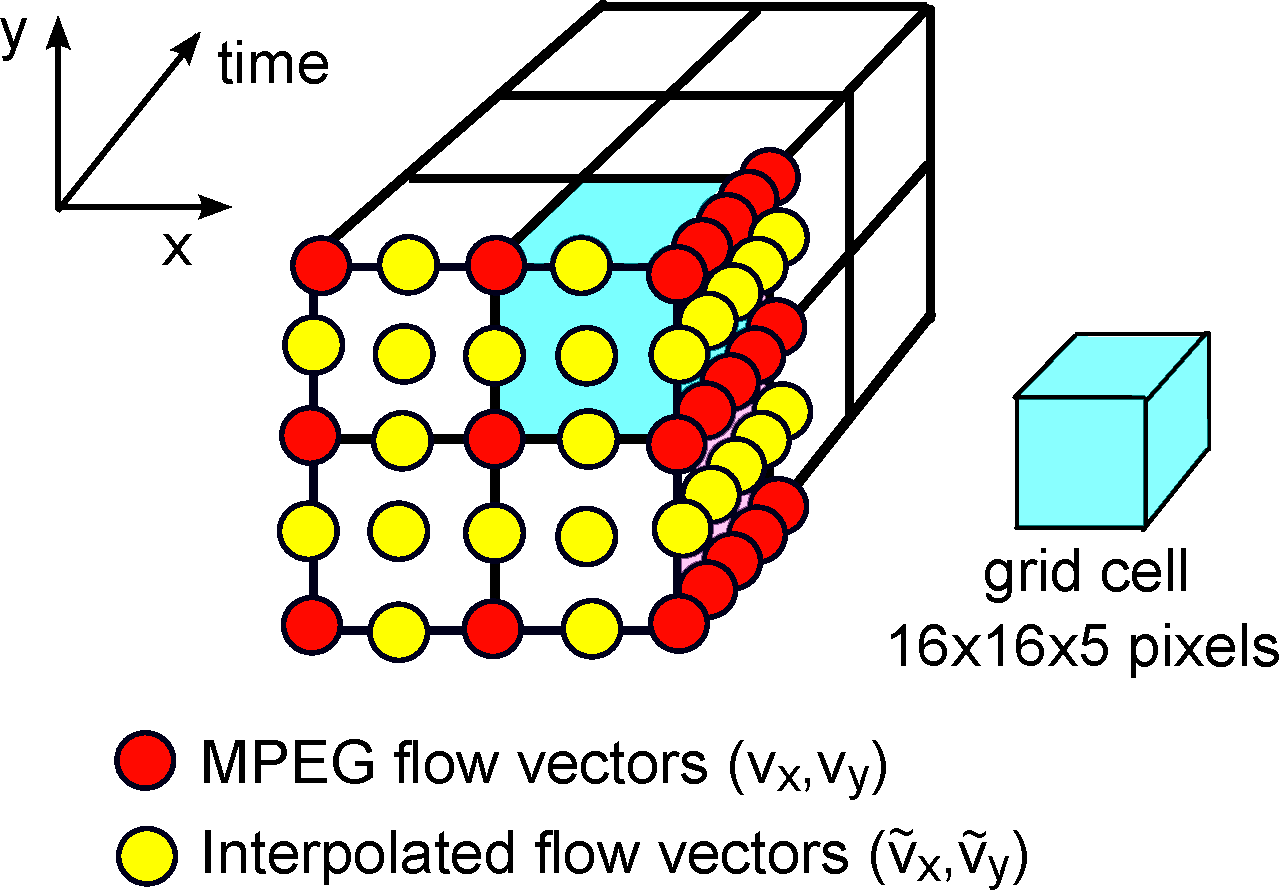
\includegraphics[width=.6\linewidth]{cvpr14_figures/CD-descriptor2.pdf}
\caption[MPEG flow video descriptor]{MPEG flow (MF) video descriptor defined at positions of MPEG flow vectors. Each $2\times2\times3$ descriptor cell is accumulated from quantized values of original and interpolated flow vectors indicated by the red and yellow circles respectively.\vspace{-.6cm}}
\label{fig:CDdescriptor}
\end{center}
\end{figure}


\begin{figure*}[!t]
\begin{center}
\vspace{-.6cm}
%\begin{tabular}{cccccc}
%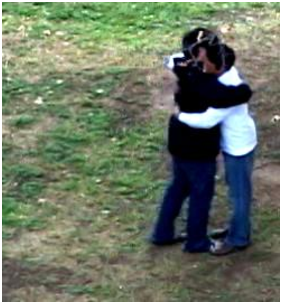
\includegraphics[scale=0.2]{cvpr14_figures/dataset_thumb/uti/crop_class1.pdf} & 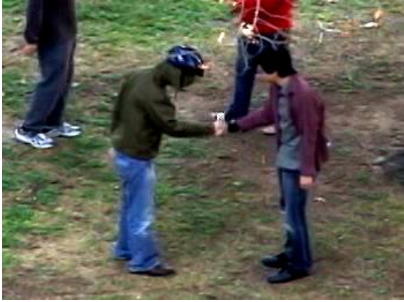
\includegraphics[scale=0.2]{cvpr14_figures/dataset_thumb/uti/crop_class2.pdf} & 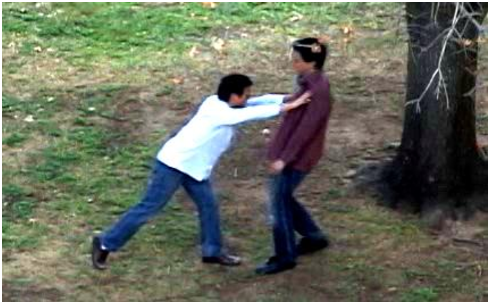
\includegraphics[scale=0.2]{cvpr14_figures/dataset_thumb/uti/crop_class3.pdf} & 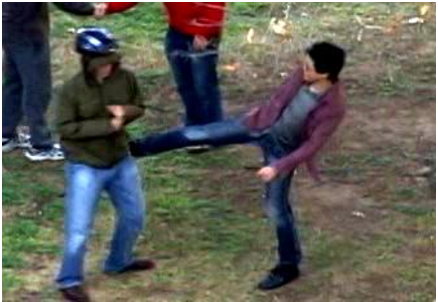
\includegraphics[scale=0.2]{cvpr14_figures/dataset_thumb/uti/crop_class4.pdf} & 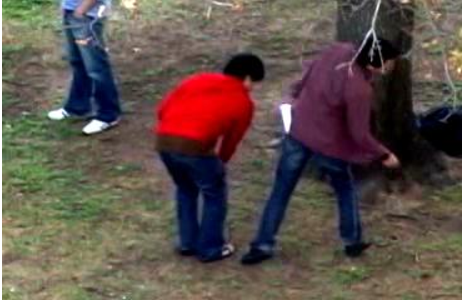
\includegraphics[scale=0.2]{cvpr14_figures/dataset_thumb/uti/crop_class5.pdf} & 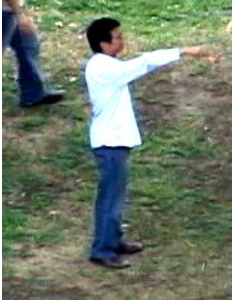
\includegraphics[scale=0.2]{cvpr14_figures/dataset_thumb/uti/crop_class6.pdf} \\
%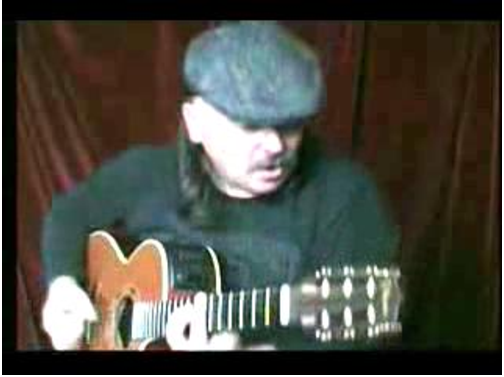
\includegraphics[scale=0.2]{cvpr14_figures/dataset_thumb/ucf/crop_class1.pdf} & 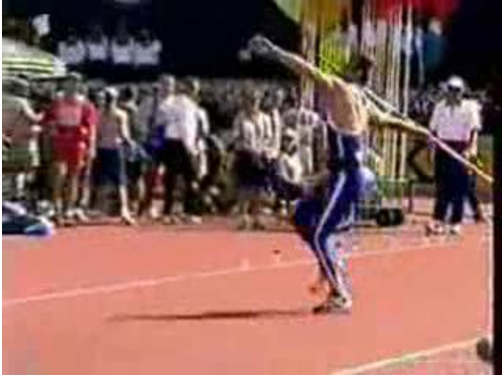
\includegraphics[scale=0.2]{cvpr14_figures/dataset_thumb/ucf/crop_class2.pdf} & 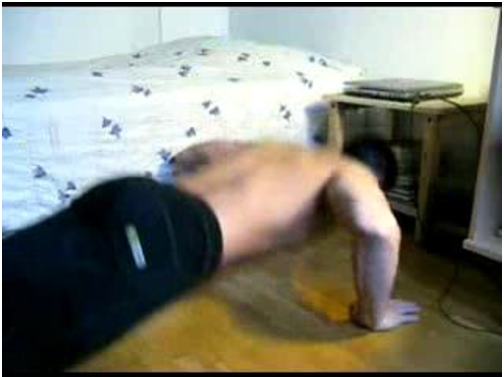
\includegraphics[scale=0.2]{cvpr14_figures/dataset_thumb/ucf/crop_class3.pdf} & 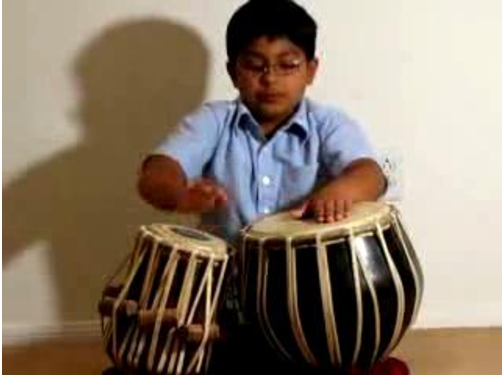
\includegraphics[scale=0.2]{cvpr14_figures/dataset_thumb/ucf/crop_class4.pdf} & 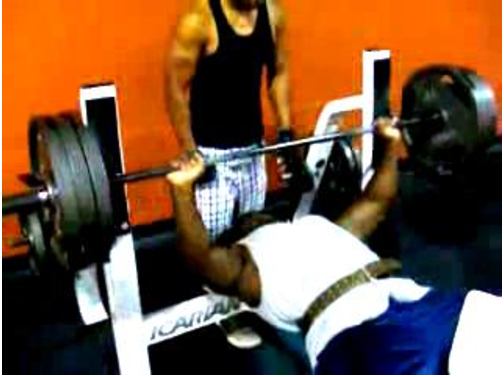
\includegraphics[scale=0.2]{cvpr14_figures/dataset_thumb/ucf/crop_class5.pdf} & 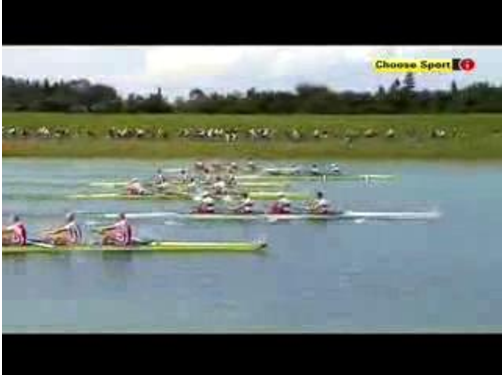
\includegraphics[scale=0.2]{cvpr14_figures/dataset_thumb/ucf/crop_class6.pdf} \\
%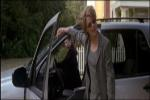
\includegraphics[height=1cm]{cvpr14_figures/dataset_thumb/hwd/class1.jpg} & 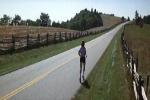
\includegraphics[height=1cm]{cvpr14_figures/dataset_thumb/hwd/class2.jpg} & 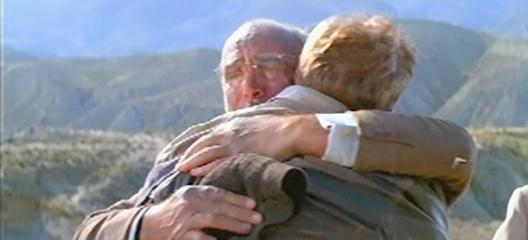
\includegraphics[height=1cm]{cvpr14_figures/dataset_thumb/hwd/class3.jpg} & 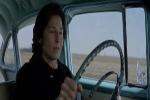
\includegraphics[height=1cm]{cvpr14_figures/dataset_thumb/hwd/class4.jpg} & 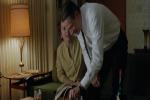
\includegraphics[height=1cm]{cvpr14_figures/dataset_thumb/hwd/class5.jpg} & 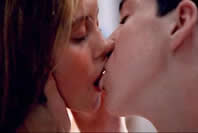
\includegraphics[height=1cm]{cvpr14_figures/dataset_thumb/hwd/class6.jpg} \\
%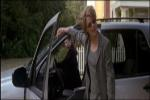
\includegraphics[height=1.61cm]{cvpr14_figures/dataset_thumb/hwd/class1.jpg} 
%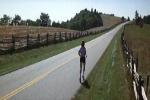
\includegraphics[height=1.61cm]{cvpr14_figures/dataset_thumb/hwd/class2.jpg} 
%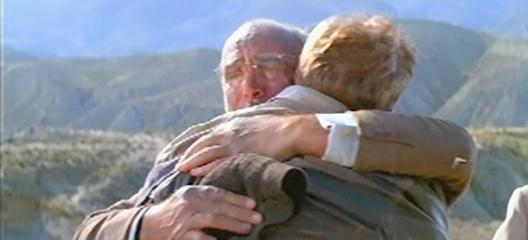
\includegraphics[height=1.61cm]{cvpr14_figures/dataset_thumb/hwd/class3.jpg}  
%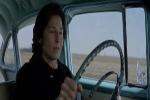
\includegraphics[height=1.61cm]{cvpr14_figures/dataset_thumb/hwd/class4.jpg}
%\includegraphics[height=1.61cm]{cvpr14_figures/dataset_thumb/hwd/class5.jpg}
%\includegraphics[height=1.61cm]{cvpr14_figures/dataset_thumb/hwd/class6.jpg} \\
%\includegraphics[scale=0.305]{cvpr14_figures/dataset_thumb/ucf/crop_class1.pdf}
%\includegraphics[scale=0.305]{cvpr14_figures/dataset_thumb/ucf/crop_class2.pdf}
%\includegraphics[scale=0.305]{cvpr14_figures/dataset_thumb/ucf/crop_class3.pdf} 
%\includegraphics[scale=0.305]{cvpr14_figures/dataset_thumb/ucf/crop_class4.pdf} 
%\includegraphics[scale=0.305]{cvpr14_figures/dataset_thumb/ucf/crop_class5.pdf} 
%\includegraphics[scale=0.305]{cvpr14_figures/dataset_thumb/ucf/crop_class6.pdf} \\
%\includegraphics[scale=0.4]{cvpr14_figures/dataset_thumb/uti/crop_class1.pdf} 
%\includegraphics[scale=0.4]{cvpr14_figures/dataset_thumb/uti/crop_class2.pdf} 
%\includegraphics[scale=0.4]{cvpr14_figures/dataset_thumb/uti/crop_class3.pdf} 
%\includegraphics[scale=0.4]{cvpr14_figures/dataset_thumb/uti/crop_class4.pdf} 
%\includegraphics[scale=0.4]{cvpr14_figures/dataset_thumb/uti/crop_class5.pdf} 
%\includegraphics[scale=0.4]{cvpr14_figures/dataset_thumb/uti/crop_class6.pdf} \\
\includegraphics[height=1.3cm]{cvpr14_figures/dataset_thumb/hwd/class1.jpg} 
\includegraphics[height=1.3cm]{cvpr14_figures/dataset_thumb/hwd/class2.jpg} 
\includegraphics[height=1.3cm]{cvpr14_figures/dataset_thumb/hwd/class3.jpg}  
\includegraphics[height=1.3cm]{cvpr14_figures/dataset_thumb/hwd/class4.jpg}
\includegraphics[height=1.3cm]{cvpr14_figures/dataset_thumb/hwd/class5.jpg}
\includegraphics[height=1.3cm]{cvpr14_figures/dataset_thumb/hwd/class6.jpg} \\
\includegraphics[scale=0.25]{cvpr14_figures/dataset_thumb/ucf/crop_class1.pdf}
\includegraphics[scale=0.25]{cvpr14_figures/dataset_thumb/ucf/crop_class2.pdf}
\includegraphics[scale=0.25]{cvpr14_figures/dataset_thumb/ucf/crop_class3.pdf} 
\includegraphics[scale=0.25]{cvpr14_figures/dataset_thumb/ucf/crop_class4.pdf} 
\includegraphics[scale=0.25]{cvpr14_figures/dataset_thumb/ucf/crop_class5.pdf} 
\includegraphics[scale=0.25]{cvpr14_figures/dataset_thumb/ucf/crop_class6.pdf} \\
\includegraphics[scale=0.19]{cvpr14_figures/dataset_thumb/hmdb/class1.png}
\includegraphics[scale=0.19]{cvpr14_figures/dataset_thumb/hmdb/class2.png}
\includegraphics[scale=0.19]{cvpr14_figures/dataset_thumb/hmdb/class3.png} 
\includegraphics[scale=0.19]{cvpr14_figures/dataset_thumb/hmdb/class4.png} 
\includegraphics[scale=0.19]{cvpr14_figures/dataset_thumb/hmdb/class5.png} 
\includegraphics[scale=0.19]{cvpr14_figures/dataset_thumb/hmdb/class6.png} \\
\includegraphics[scale=0.32]{cvpr14_figures/dataset_thumb/uti/crop_class1.pdf} 
\includegraphics[scale=0.32]{cvpr14_figures/dataset_thumb/uti/crop_class2.pdf} 
\includegraphics[scale=0.32]{cvpr14_figures/dataset_thumb/uti/crop_class3.pdf} 
\includegraphics[scale=0.32]{cvpr14_figures/dataset_thumb/uti/crop_class4.pdf} 
\includegraphics[scale=0.32]{cvpr14_figures/dataset_thumb/uti/crop_class5.pdf} 
\includegraphics[scale=0.32]{cvpr14_figures/dataset_thumb/uti/crop_class6.pdf} \\
%\end{tabular}
\smallskip
\caption[Sample frames from action recognition datasets]{Sample frames from action recognition datasets. From top to bottom: Hollywood2~\cite{Marszalek09}, UCF50~\cite{Reddy12}, HMDB51~\cite{Kuehne11}, UT-Interaction~\cite{Ryoo10}.\vspace{-.5cm}}
\label{fig:datasets}
\end{center}
\end{figure*}



